\section{GitEye}
\begin{frame}[allowframebreaks]
\frametitle{GitEye}
 
\begin{itemize}
 \item koristan za velike kompanije - lakoćom se upravlja važnim projektima
 \item povlači repozitorije gdje god se oni nalazili
 \item poseban modul praćenja promjena datoteka - više ljudi radi na dokumentu bez da smetaju jedno drugome
 \item integrira se s uslugama razvojnih programera treće strane kako bi se olakšao proces upravljanja projektima
 \framebreak
 \item korisne i user-friendly značajke:
 		\item izvrsno sučelje
 		\item pristupačan pregled povijesti
 		\item besplatan i učestali update aplikacije
\end{itemize}

\begin{figure}
	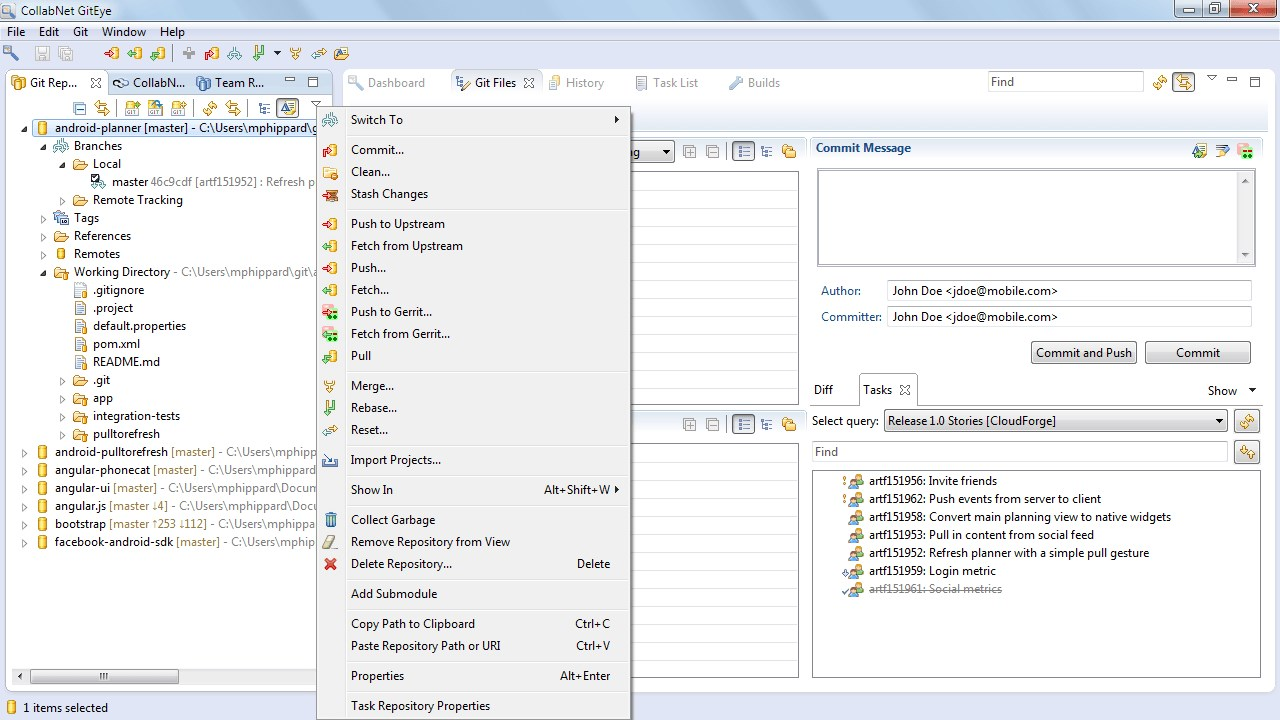
\includegraphics[width=0.9\linewidth]{images/git-eye.jpeg}
\end{figure}
\end{frame}
